\section{Pourcentage d'évolution et ajustement}

Les volumes des ventes (en milliers de boites) d'un médicament mis sur le marché en 2008 sont donnés par l'extrait de feuille de calcul ci-dessous.

\begin{center}
	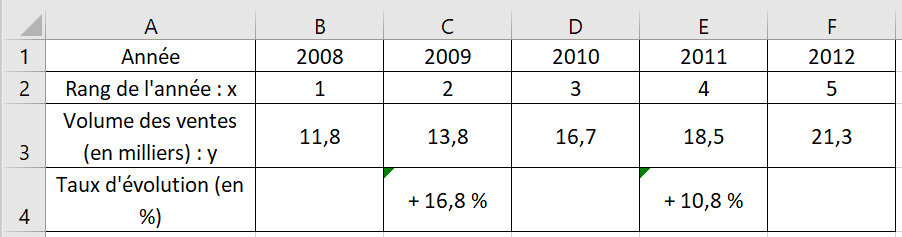
\includegraphics[scale=0.4]{tab}
\end{center}

Une représentation du nuage de points est donnée en annexe, à rendre avec la copie.

\begin{questions}
	\question 
		\begin{parts}
			\part Calculer le pourcentage d'évolution entre 2009 et 2010, le résultat sera arrondi à l'unité.
			
			\part Donner une formule qui, entrée dans la cellule $C4$, permet, par recopie vers la droite d'obtenir les pourcentages d'évolution voulus dans la plage $C4:F4$.
			
		\end{parts}
	
	\question On envisage de modéliser par un ajustement affine l'évolution du volume des ventes de ce produit. On se propose d'ajuster le nuage par la droite $(d)$ passant par les points  $A(1;\num{11.8})$ et $B(5;\num{21.3})$. Déterminer l'équation de la droite $(d)$ et la tracer sur le graphique.
		
	
	\question En utilisant cet ajustement :
		\begin{parts}
			\part Déterminer graphiquement une estimation du nombre de boites de médicaments que l'on vendra en 2013. %On fera apparaitre les traces nécessaires à la lecture sur le graphique.
			
			\part Calculer à l'aide de l'équation $y = \num{2.375}x + \num{9.425}$, une estimation du nombre de boites que l'on vendra en 2016.
		\end{parts}
\end{questions}

\begin{center}
	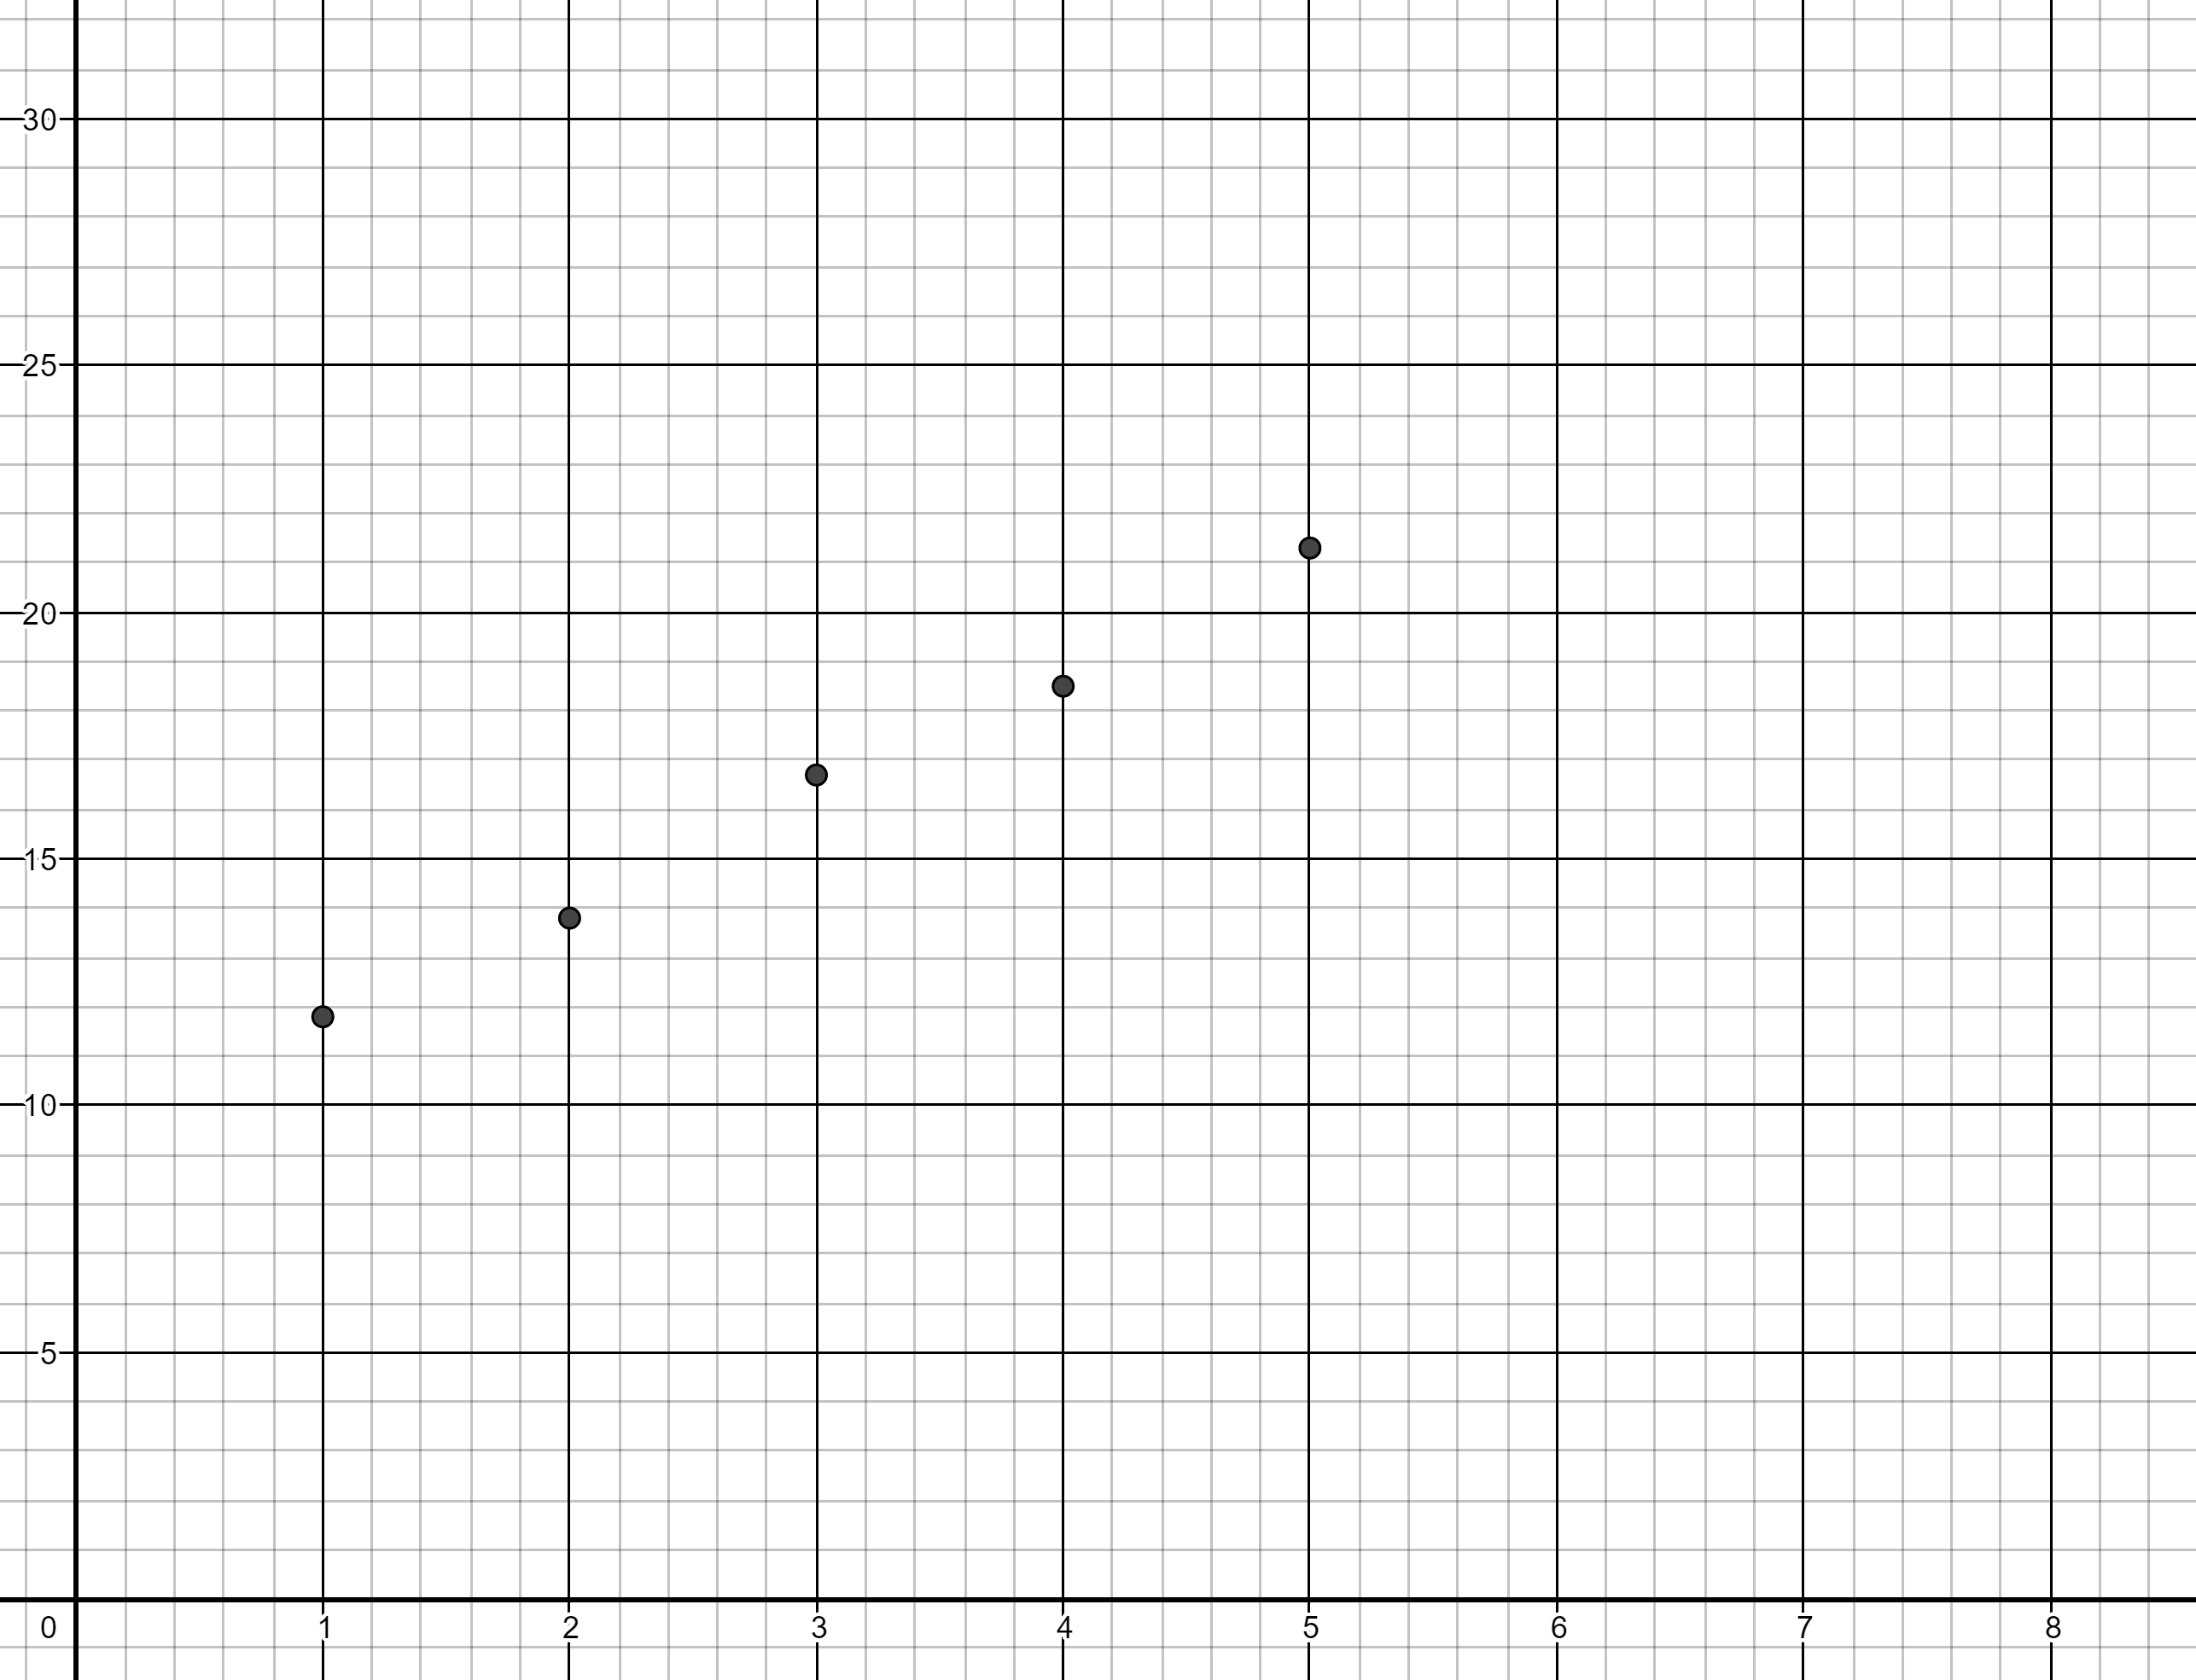
\includegraphics[scale=0.20]{graph}
\end{center}